% PACKAGES INCLUDED HERE 
% DO NOT NEED TO CHANGE
\documentclass[conference]{IEEEtran}
%\IEEEoverridecommandlockouts
% The preceding line is only needed to identify funding in the first footnote. If that is unneeded, please comment it out.
\usepackage{cite}
\usepackage{amsmath,amssymb,amsfonts}
\usepackage{algorithmic}
\usepackage{graphicx}
\usepackage{textcomp}
\def\BibTeX{{\rm B\kern-.05em{\sc i\kern-.025em b}\kern-.08em
    T\kern-.1667em\lower.7ex\hbox{E}\kern-.125emX}}
\begin{document}

% TITLE GOES HERE

\title{Neural Nets to Score Colliding Galaxy Models\\}


% AUTHOR NAMES GOES HERE
\author{
\IEEEauthorblockN{Shawn Mace}
\IEEEauthorblockA{\textit{Department of Computer Science} \\
\textit{Middle Tennessee State University}\\
Murfreesboro, United States \\
sdm2w@mtmail.mtsu.edu}\\
\IEEEauthorblockN{Derrick Reckers}
\IEEEauthorblockA{\textit{Department of Computer Science} \\
\textit{Middle Tennessee State University}\\
Murfreesboro, United States \\
dmr3p@mtmail.mtsu.edu}\\
\and
\IEEEauthorblockN{Aric Moilanen}
\IEEEauthorblockA{\textit{Department of Physics and Astronomy} \\
\textit{Middle Tennessee State University}\\
Murfreesboro, United States \\
atm4w@mtmail.mtsu.edu}\\
\IEEEauthorblockN{Jarrett Shaver}
\IEEEauthorblockA{\textit{Department of Computer Science} \\
\textit{Middle Tennessee State University}\\
Murfreesboro, United States \\
Jarrett.shaver@gmail.com}\\
\and
\IEEEauthorblockN{Matthew Ogden}
\IEEEauthorblockA{\textit{Computational Science, PhD Program} \\
\textit{Middle Tennessee State University}\\
Murfreesboro, United States \\
mbo2d@mtmail.mtsu.edu}\\
\IEEEauthorblockN{Devon Wilson}
\IEEEauthorblockA{\textit{Department of Computer Science} \\
\textit{Middle Tennessee State University}\\
Murfreesboro, United States \\
email address}\\
}
\maketitle

% ABSTRACT 

\begin{abstract}
This document is a model and instructions for \LaTeX.
This and the IEEEtran.cls file define the components of your paper [title, text, heads, etc.]. *CRITICAL: Do Not Use Symbols, Special Characters, Footnotes, 
or Math in Paper Title or Abstract.
\end{abstract}


% KEYWORDS

\begin{IEEEkeywords}
component, formatting, style, styling, insert
\end{IEEEkeywords}

% INTRODUCTION SECTION
\section{Introduction}

When two galaxies merge, it causes a drastic change in the
evolution of the resulting galaxy. Understanding ongoing
collisions in the night sky, will aid scientists in their exploration
to uncover more about merging galaxies. Unfortunately,
information such as orbital velocities, orientations, and mass-ratios between the two galaxies cannot be obtained from
observation alone.

To obtain this information, past research has looked into
modeling the dynamics of interacting galaxies and developing
galactic models to simulate galaxy interactions. By finding
models and analyzing how well they fit known observations of
galaxies, models that “best fit” observations could reflect the
true parameters for the galaxy collisions.

This project takes data from galactic models and associated
human fitness scores, with the goal to develop several Neural
Network Tools that help scientists better understand this
data, and develop a machine fitness score that matches the
human fitness score. By having theses tools, scientists can
quicken the search to find those well-fitting models, explore
the galactic model parameter space, and hopefully find the
true dynamic parameters for observable galaxy collisions.

% BACKGROUND SECTION
\section{Background}

Our project is based on several pieces of research. First is
the work of Toomre and Toomre who demonstrated merging
galaxies would cause distinct tidal distortions \cite{Toomre}. These tidal
distortions often result in the galaxies forming “bridges” and
“tails”, star regions that appear to bridge the gap between the
two galaxies, and arc away from each other. Toomre and
Toomre performed a variety of simulations showing that the
gravitation interactions caused these distinct shapes \cite{Toomre}.

Second is the work of SPAM. SPAM is O(n) public release
software that builds upon the restricted three-body model to
simulate galactic models merging. SPAM takes galactic
models and simulates the two galaxies merger. In addition,
point particles are added, undergoing realistic tidal distortions
and produce the iconic bridge and tail shapes \cite{WallinJSPAM}.

Lastly, most of our data has origins from Galaxy Zoo:
Mergers. Galaxy Zoo: Mergers is a citizen scientist effort to
explore the unknown parameter space for the galactic models.
Using the quick efficiency of SPAM to visual the final shape of
galactic models, millions of galactic models were simulated
and views by thousands of volunteers. Citizen scientists would
select models with a similar shape to the target image the
models are attempting to represent. From there, those
selected models went through a tournament like competition
with other models to receive the human fitness score. The
citizen scientist would choose the galactic model whose shape
better matches the target images. After going through the
tournament, all the models would have an associated fitness
scores \cite{WallinGalaxyZoo}.

The galactic models and their associated human fitness
score are what were used in this project. The human fitness
scores were directly applied, while the galactic models had to
be visualized again. The galactic models were sent through
SPAM again with a larger number of particles to obtain a 
higher resolution image of the colliding galaxies. These model
images and the human fitness scores are used \cite{WallinJSPAM}\cite{WallinGalaxyZoo}.


% METHODS SECTION
\section{Methods}

\subsection{Data}

\begin{figure}[htbp]
\centerline{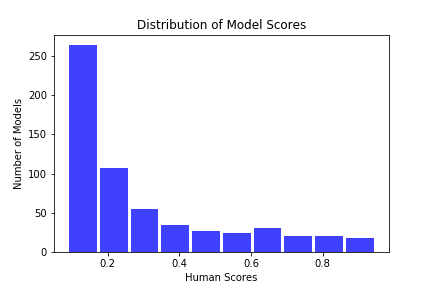
\includegraphics[width=0.75\linewidth]{./Images/distribution.png}}
\caption{Distribution of sample models across a range of human scores from 0-1.}
\label{fig:distribution}
\end{figure}

We chose one of the 62 pairs of galaxies and pulled the associated data. This set consisted of 1294 grayscale model images in .png format and their associated human scores in a text file. The set was already sorted in descending order by score. However, we realized that this data was heavily skewed towards worse models, with more than half of the models having scores below 0.10. In an effort to combat overfitting on bad model images, we used only the first 600 images, which, while still skewed towards worse models (see Fig. \ref{fig:distribution}), presented a much more evenly distributed data set.

\begin{figure}[htbp]
\centerline{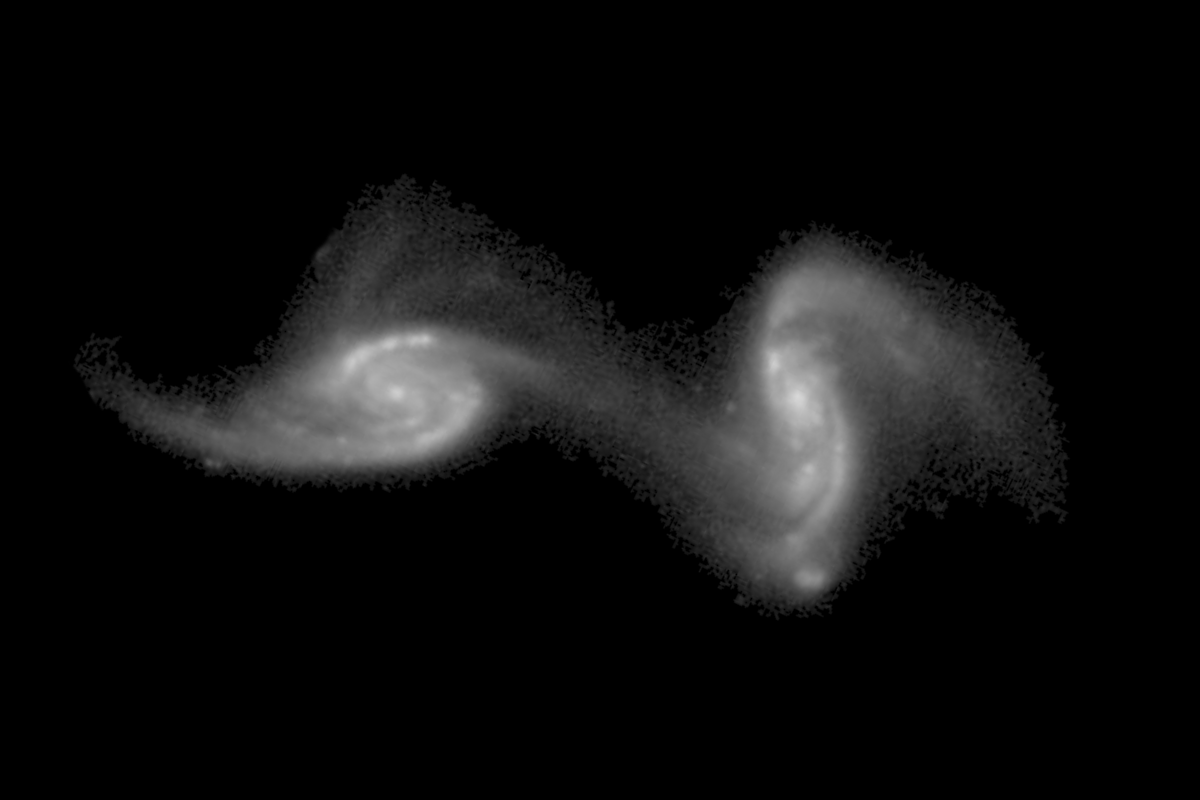
\includegraphics[width=0.75\linewidth]{./Images/target.png}}
\caption{The chosen colliding galaxy pair for this project. A higher model score should represent a model that closely resembles this image.}
\label{fig:TargetGalaxy}
\end{figure}

The images and scores were read in using a technique similar to the MNIST problem presented in OLA 6. The main difference being that the grab\_image function was modified to read in our images as greyscale rather than full RGB and at a reduced resoultion of 100x100. We then shuffled the images, taking care to manipulate them in such a way that the scores would retain the same index as their respective images. This shuffling ensured that models of similar scores would be randomly distributed, preventing the model from learning soley on one quality of model at a time. 

The 600 shuffled images were then split into a training and validation set consisting of 510 images and a testing set with the remaining 90 images. When training our nets, a validation split of 0.3 was used, resulting in the nets training on 357 images and validating on the remaining 153.

\subsection{Single Layer Neural Net}

For the single layer net, the images were flattened to 1D arrays then passed into a single dense layer. This layer was given an input size of 1 and a Softmax activation function in order to return a single score between 0 and 1. This net, and the nets discussed below, were all compiled with mean squared error, which is the best fit for regression problems, as the loss parameter.

In training our nets, we found that a small batch size was an absolute necessity for decent learning, most likely due to the small data set and skew towards worse models. We used a batch size of 4 for all of the nets discussed in this project.

\subsection{Convolutional Neural Net}

In our second net, we attempted to utilize the superior image recognition characteristics of a convolutional neural net. As a base, we used the convolutional neural net used on the cat problem in OLA 6. In this net, there are two 2D convolution layers that feed into a pooling layerThe main changes made were to kernel size and the final dense layer. There are two 2D convolution layers use a standard ReLu activation function, which are then followed by pooling and dropout layer. It is the passed into a flattening layer and a single dense layer, still with a ReLu activation function, before passing though a final dropout layer and into the final dense layer. The main changes we made to this architecture from OLA 6 were in terms of kernel size, unit size of the dense and convolution layers, and the setup of the final dense layer. 

We adjusted the kernel sizes to be slightly larger. This was done in an attempt to better capture what we believed were the most important characteristics of the image, namely the tidal distortions around the edges of each galaxy and the bridge, or lack thereof, between the galaxies. The unit sizes in the convolution layers were made smaller in order to fit our relatively small data set. Without doing this, we experienced drastic overfitting or no training at all. The final dense layer was also changed to match our plan for a regression model. The input for the final layer was reduced to 1 and the activation changed to Softmax in order to return a single score between 0 and 1 for the model image.

\begin{figure}[htbp]
\centerline{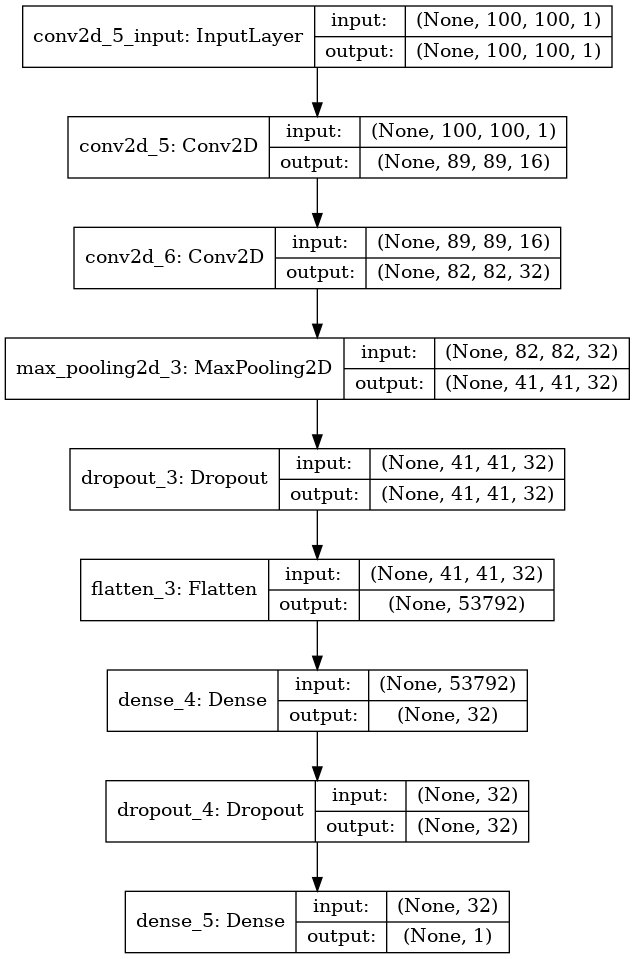
\includegraphics[width=0.5\linewidth]{./Images/convNet.png}}
\caption{Layout of the convolutional neural net}
\label{fig:ConvNetArchitecture}
\end{figure}


% RESULTS SECTION
\section{Results}

\subsection{Single Layer Net Results}

\begin{figure}[htbp]
\centerline{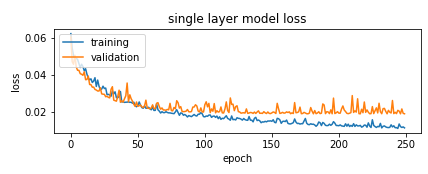
\includegraphics[width=0.75\linewidth]{./Images/SingleModelLoss.png}}
\caption{Loss (Mean Squared Error) for the single layer net over 120 epochs}
\label{fig:SingleModelLoss}
\end{figure}

Shown in Fig. \ref{fig:SingleModelLoss} is the training and validation loss history over 120 epochs. At the end of 120 epochs, the model had decreased to a MSE loss of 0.012 for the training data and 0.019 for the validation data. We can also plainly see the overfitting the plagued both of our neural nets, regardless of the hyperparameter tuning we performed to try to remove it.

\begin{figure}[htbp]
\centerline{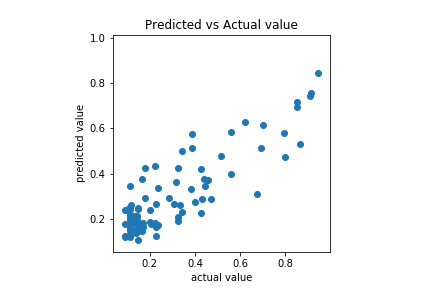
\includegraphics[width=0.75\linewidth]{./Images/SinglePredictedVAct.png}}
\caption{Predicted values generated by single layer net vs actual value}
\label{fig:SinglePredictedVAct}
\end{figure}

Fig. \ref{fig:SinglePredictedVAct} shows the values predicted by the single layer net on the 90 testing images verus their human scores. We see a linear correlation between the two, which is what we hoped to observe. A perfect linear correlation would have meant that the model was guessing exactly the same as the human score.

\begin{figure}[htbp]
\centerline{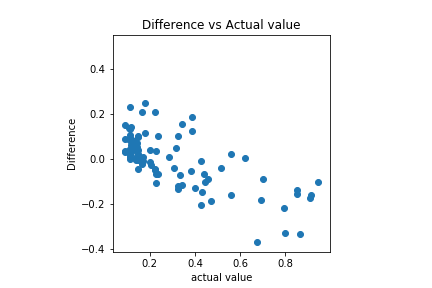
\includegraphics[width=0.75\linewidth]{./Images/SingleDiffVAct.png}}
\caption{Difference between predicted values generated by single layer net and actual values vs actual value}
\label{fig:SingleDiffVAct}
\end{figure}

Fig. \ref{fig:SingleDiffVAct} shows the difference between the values predicted by the single layer net for the 90 test images and their human scores versus the human scores. From this plot, it is easy to see that the net had a tendency to overscore models with low human scores and underscore models with high human scores. We can also see that the most accurate predictions occured for models with lower human scores, which makes sense given the data's skew towards worse models. Over the full 90 image set, the net attained a mean difference of 0.093 between its predicted values and the human scores.

\begin{figure}[htbp]
\centerline{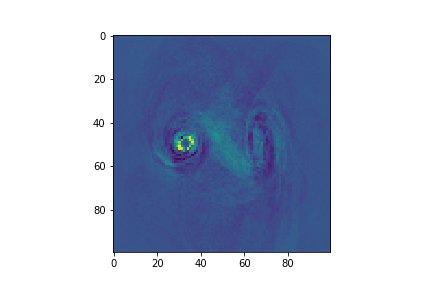
\includegraphics[width=0.75\linewidth]{./Images/singleWeights.png}}
\caption{Visualization of weights for the single layer net}
\label{fig:singleWeights}
\end{figure}

The final weights for the single layer net are shown in Fig. \ref{fig:singleWeights}. We see that the net is placing emphasis on the bridge forming between the two galaxies as well as on the tidal distortions around the edges. Interestingly, the net also thinks that the core of the left galaxy is extremely important. This may be due to the fact that all of our model images are positioned roughly the same way, and in every image there is a bright spot marking the center of a galaxy at roughly the hotspot location shown in Fig. \ref{fig:singleWeights}.

\begin{figure}[htbp]
\centerline{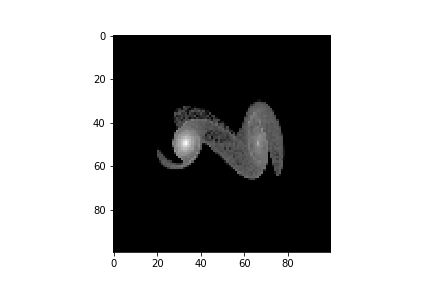
\includegraphics[width=0.75\linewidth]{./Images/SinglePredictedBest.png}}
\caption{Model that was scored the highest by the single layer neural net}
\label{fig:SinglePredictedBest}
\end{figure}


Shown in Fig. \ref{fig:SinglePredictedBest} is the model that the single layer net scored the highest (0.846). Its real human score was 0.946, so this shows good agreement between the net's perception and human perception of what the best model is. We can also visually verify that this chosen model closely resembles the target image shown in Fig. \ref{fig:TargetGalaxy}.

\subsection{Convolutional Neural Net Results}

\begin{figure}[htbp]
\centerline{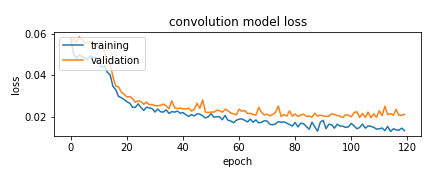
\includegraphics[width=0.75\linewidth]{./Images/ConvModelLoss.png}}
\caption{Layout of the convolutional neural net}
\label{fig:ConvModelLoss}
\end{figure}

In Fig. \ref{fig:ConvModelLoss} we see very similar learning behavior to the single layer net. Both display overfitting issues and, after 120 epochs, reach approximately the same MSE. For the convolutional net, the final MSE for the training data was 0.013 and 0.021 which is just slightly worse than the single layer net. Qualitatively, the only difference in learning behavior was the prescence of a slight plateau for the fist 10 or so epochs before the net actually began to learn quickly.

\begin{figure}[htbp]
\centerline{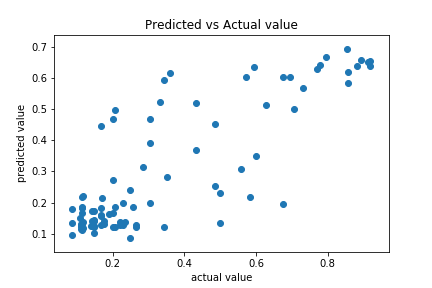
\includegraphics[width=0.75\linewidth]{./Images/ConvPredictedVAct.png}}
\caption{Predicted values generated by convolutional net vs actual value}
\label{fig:ConvPredictedVAct}
\end{figure}

Like with the single layer net, Fig. \ref{fig:ConvPredictedVAct} shows a linear correlation between the predicted values and human scores. However, as the human scores increase, we see a wider spread in predicted values when compared to the single layer net. 

\begin{figure}[htbp]
\centerline{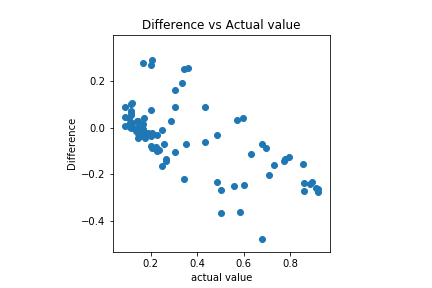
\includegraphics[width=0.75\linewidth]{./Images/ConvDiffVAct.png}}
\caption{Difference between predicted values generated by convolutional net and actual values vs actual value}
\label{fig:ConvDiffVAct}
\end{figure}

Once again, Fig. \ref{fig:ConvDiffVAct} shows that the convolutional net has a tendency to overscore worse models and underscore better models. However, when compared to the single layer net, we see a much tighter grouping of worse models (human scores $\leq0.3$) that the model was able to accurately guess with a difference of $-0.1 \leq$ Diff $\leq 0.1$. For the 90 image testing set, the convoltional net attained a mean difference of 0.112, which is slightly worse than the single layer net. 

\begin{figure}[htbp]
\centerline{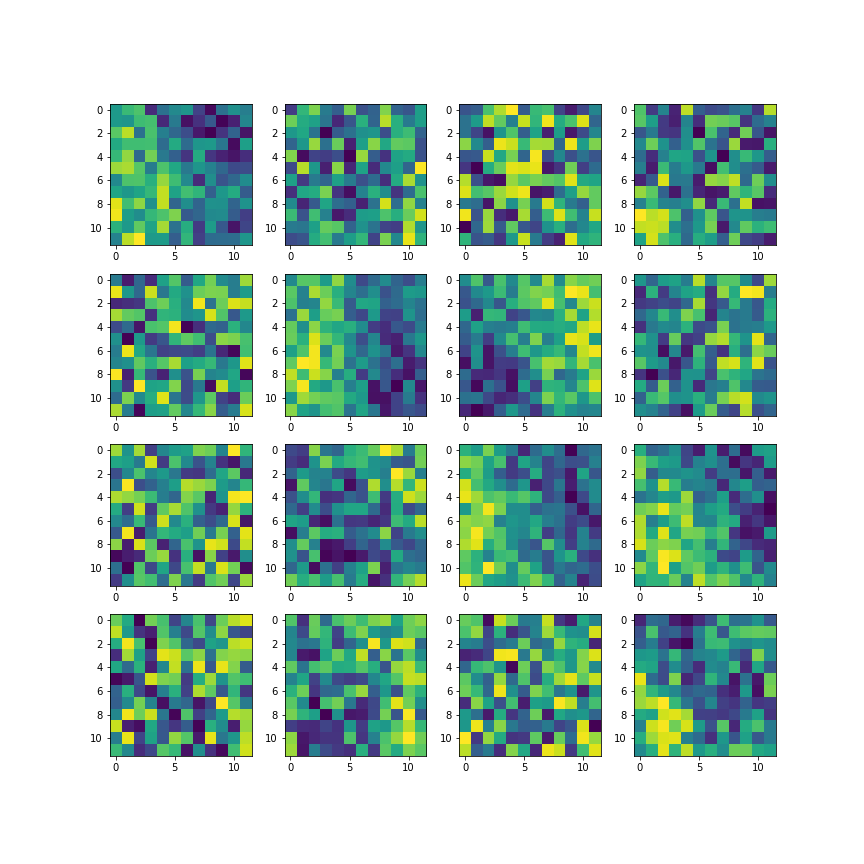
\includegraphics[width=0.75\linewidth]{./Images/convWeight1.png}}
\caption{Visualization of weights for the first convolution layer}
\label{fig:convWeight1}
\end{figure}

\begin{figure}[htbp]
\centerline{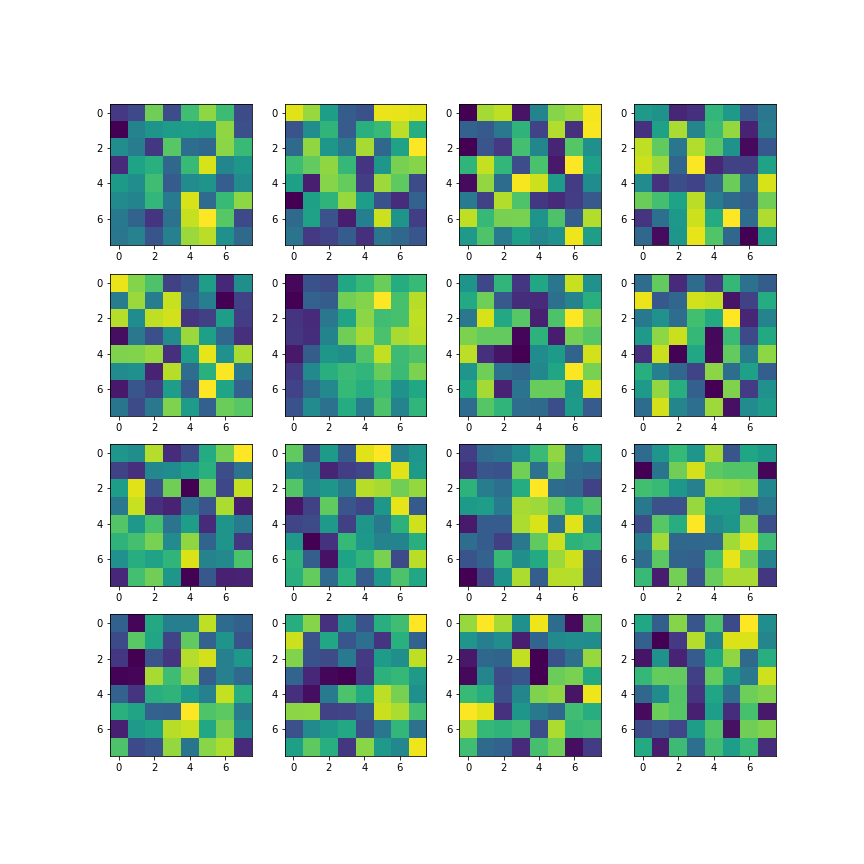
\includegraphics[width=0.75\linewidth]{./Images/convWeight2.png}}
\caption{Visualization of weights for the second convolution layer}
\label{fig:convWeight2}
\end{figure}

\begin{figure}[htbp]
\centerline{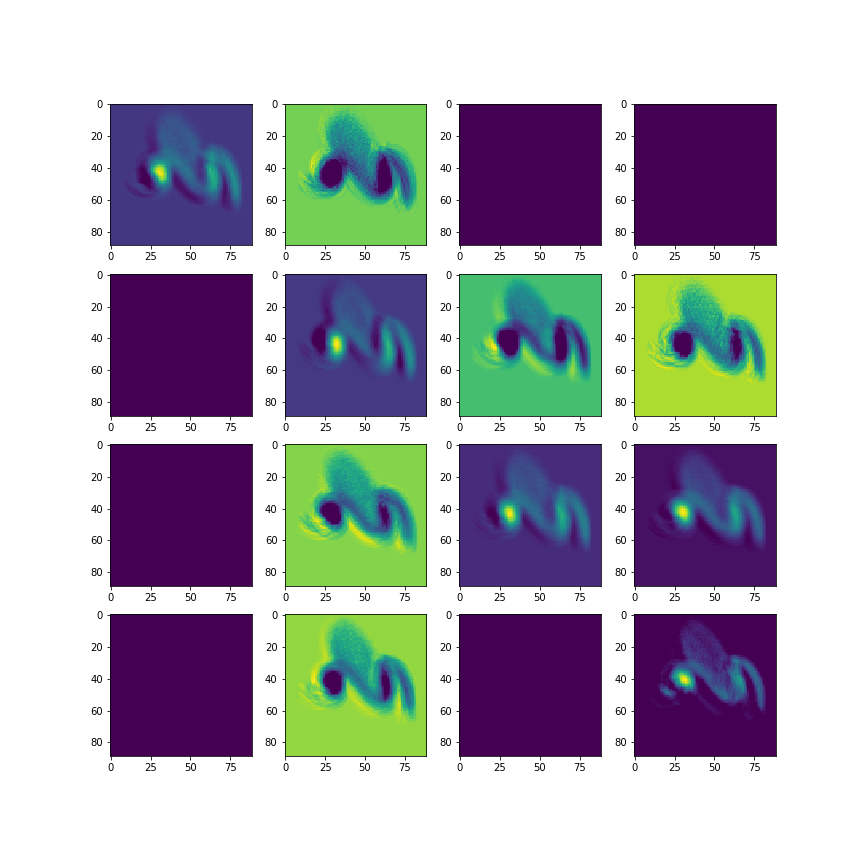
\includegraphics[width=0.75\linewidth]{./Images/layer1activations.png}}
\caption{Visualization of network activations for the first convolution layer}
\label{fig:layer1activations}
\end{figure}

Fig. \ref{fig:convWeight1} and Fig. \ref{fig:convWeight2} show the weights for the first and second convolution layers respectively. However, it is hard to glean and useful information from just these weights on their own. That is why we have shown the activations of units in the first layer in Fig. \ref{fig:layer1activations}. We can see that for this specific activation, the net was processing a model that was very similar to the target image. We can see units that are picking up the major features: galactic cores, tidal distortions, and the bridge. We can also plainly see the units that are detecting the edges of the galaxies, as well as some units that aren't really being utilized.

\begin{figure}[htbp]
\centerline{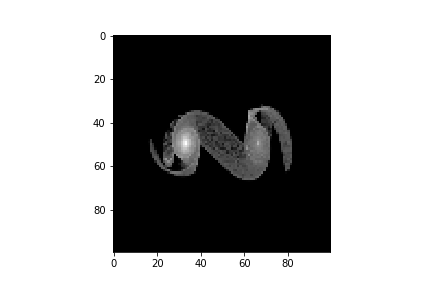
\includegraphics[width=0.75\linewidth]{./Images/ConvPredictedBest.png}}
\caption{Model that was scored the highest by the convolutional neural net}
\label{fig:ConvPredictedBest}
\end{figure}

Fig. \ref{fig:ConvPredictedBest} shows the image that was given the highest score by the convolutional net (0.695). This predicted value is significantly lower than the human score of 0.853, but it shows that the  convolutional net was still atleast somewhat successful in deciding on what the best model should look like. Once again, we can visually verify that the convolutional net's predicted best model closely resembles the target image shown in Fig. \ref{fig:TargetGalaxy}.

% DISCUSSION SECTION
\section{Discussion}

Both the single layer neural network and convolutional neural network show promise in correctly predicting how good of a fit a model is for a target galaxy collision. Both nets achieved a MSE of $\approx 0.02$ on the validation data and a mean difference of $\approx 0.1$ when tasked with predicting the scores of 90 test models. Both nets successfully chose an image out of a set of 90 that they decided was the best model for the target image. Upon visual comparison, these two chosen models very closely resemble the target galaxy collision. However, both models struggled with overfitting which can most likely be attributed to both our data set's small size and its uneven distribution of model quality. 

\begin{figure}[htbp]
\centerline{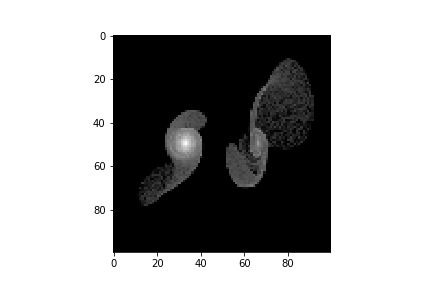
\includegraphics[width=0.75\linewidth]{./Images/ConvHumanNoiseExample.png}}
\caption{Example of a model that the convolutional net scored "poorly" when just comparing against human score.}
\label{fig:ConvHumanNoiseExample}
\end{figure}

Another factor to consider is the noise associated with the human scores. As a citizen scientist project, the models in the Galaxy Zoo: Mergers data set were ranked by people with minimal training. There are also no checks in place to prevent against people clicking though models without consideration, artificially inflating or deflating their scores. We must also acknowledge the randomness of the tournament system. It is entirely possible that some models were "unlucky" and went against rounds of exclusively good models, causing them to be scored lower than they actually should have or vice versa.

Take for example the model shown in Fig. \ref{fig:ConvHumanNoiseExample}. This was one of the convolutional net's worst predictions, with a difference of nearly 0.5 between the net's predicted score of 0.195 and the human score of 0.676. However, if we visually compare this model with the target image, one could argue that the model did not deserve such a high human score. Instead, the model might better represent a score between the net's prediction and the human score. 

Future work could pertain to the expansion of the convolutional net to include more layers. Training with these extra layers and units would necessitate a larger data set, hopefully with a more even distribution of model quality. We believe that such a net would obtain better results than either of the nets described in this paper.  Also, the nets we created for this paper could be applied to the other 61 galaxy pairs, and, with enough training, possibly eliminate the need for further human rankings. This would allow for new models to be created and scored much faster than they have been previously. 


% REFERENCES
% THIS IS CREATED AUTOMATICALLY
\bibliographystyle{IEEEtran}
\bibliography{references} % change if another name is used for References file

\end{document}
